\section{Evaluation: speed, capacity, and distributed execution}
\label{sec:evaluation}
The evaluation measures runtime performance and allocated memory against matched
Torch/PyG implementations, single-GPU capacity with storage offload, and the
latency of distributed graph execution.
Appendix~\ref{app:edge-nn} provides a differentiable EdgeNN example and a
Torch forward/gradient reference.

\subsection{Setup and comparison boundaries}
\label{sec:experimental-setup}
The single-GPU host has a Ryzen 7 255, approximately 44 GiB RAM, local NVMe
storage and an RTX 5070 Ti with 16 GiB device memory (driver 595.84).
The Torch path uses Torch 2.11.0+cu128, Triton 3.6.0, PyG 2.8.0.post1 and
pyg-lib 0.9.0+pt211cu128. The second host supplies an RTX 4070 Ti SUPER with
16 GiB under Ubuntu/WSL. Existing services remain running, occupying roughly
3 GiB locally and 12 GiB remotely. These are shared hosts, not dedicated,
clock-locked machines. GPU memory here means device memory; these consumer
GPUs use GDDR. Distributed communication uses NCCL 2.28.9 with its Socket
transport across the two hosts. The reproduction archive specifies the network configuration.

Inputs, dimensions, precision, outputs and graph semantics are matched within
each comparison. All measurements are FP32 forward evaluations, not training
iterations. Performance comparisons use ordinary Torch tensors and public Tiga
calls; paging and distributed experiments use native tensors. Timers cover synchronized host wall
time through completed output, with numerical validation outside the timer.
First compilation, warm execution and profiling have separate scopes. Speedup is
$$
 S = \frac{T_{\mathrm{matched\ baseline}}}{T_{\mathrm{Tiga}}}.
$$
Values below one indicate slowdown. Source/compiler hashes, commands, versions
and raw samples accompany each experiment's source snapshot.

\subsection{Runtime performance and memory efficiency}
\label{sec:performance}
Three workloads isolate different uses of the graph abstraction:
\begin{itemize}
\item Stored CSR: degree 32, 32 features, weighted neighbor sum; 8,192,
32,768 and 131,072 nodes. Peers are \code{torch.sparse.mm} and PyG
\code{MessagePassing} with COO gather--scatter. CSR setup is untimed; PyG's
required COO representation is included in its memory. The sparse peer prevents
one COO path from standing in for all optimized PyG execution.
\item Dynamic radius: scalar distance-weighted sum, nominal degree 32;
8,192, 32,768 and 131,072 points. Every call copies one of two different coordinate
snapshots, rebuilds the relation and consumes it. Peers are PyG's radius builder
plus COO message passing and pure Torch chunked-distance CSR construction plus
Torch sparse multiplication. The generated path avoids accepted-edge, distance and
edge-message arrays.
\item Dynamic exact kNN: scalar neighbor sum, $k=16$; 1,024, 4,096 and 16,384
points, extended to 32,768, 65,536 and 131,072 points. The practical peer is PyG's
kNN builder plus COO message passing. The pure Torch peer computes direct squared
distances in row chunks, selects top-k, then gathers and sums features.
Neither Torch baseline calls a Tiga graph builder or uses approximate search.
\end{itemize}

Both dynamic snapshots undergo complete edge-set comparison between the explicit
reference and PyG before timing. Radius coordinates use a binary grid and a
cutoff between squared-distance levels to avoid ambiguous FP32 boundaries.
The radius neighbor cap is 128; the complete comparison establishes that it
truncates neither snapshot. kNN reference distances use direct differences,
not the matrix-product identity. Every timed output is checked at relative and
absolute tolerance $3\cdot10^{-4}$. Coordinates actually change; unchanged-input
cache lookup is not counted as rebuilding. These generated dynamic paths use
scalar features, not wide-feature edge networks.

The two Torch graph builders bound each distance block to 16,777,216 pairs
(64 MiB for one FP32 distance plane; multiple temporary planes may coexist).
They still inspect all candidate pairs and materialize the complete accepted
relation. At 131,072 points an unchunked distance plane alone would require
64 GiB; chunking permits a real measured baseline instead of a predicted OOM.
This is an eager all-pairs implementation, not an optimized spatial index or a
claim that Torch cannot express a better algorithm.

Each of 36 configurations runs in a fresh process, with provider order randomized
across the matrix, four warmups and ten checked timed calls. Curves show median
and sample range, not cross-process confidence intervals. Peak Torch-allocated
GPU bytes include live inputs, coordinate fixtures, output, provider-specific
representations and temporary tensors. They exclude allocator reserve, CUDA
context/module storage and other processes. Counters are reset per measured
call after warmup; reserved-memory peaks are not substituted for allocation.
Separate largest-shape audits found zero additional Tiga-native device-buffer
allocations on each of the three Torch paths.

\begin{figure}[htbp]
\centering
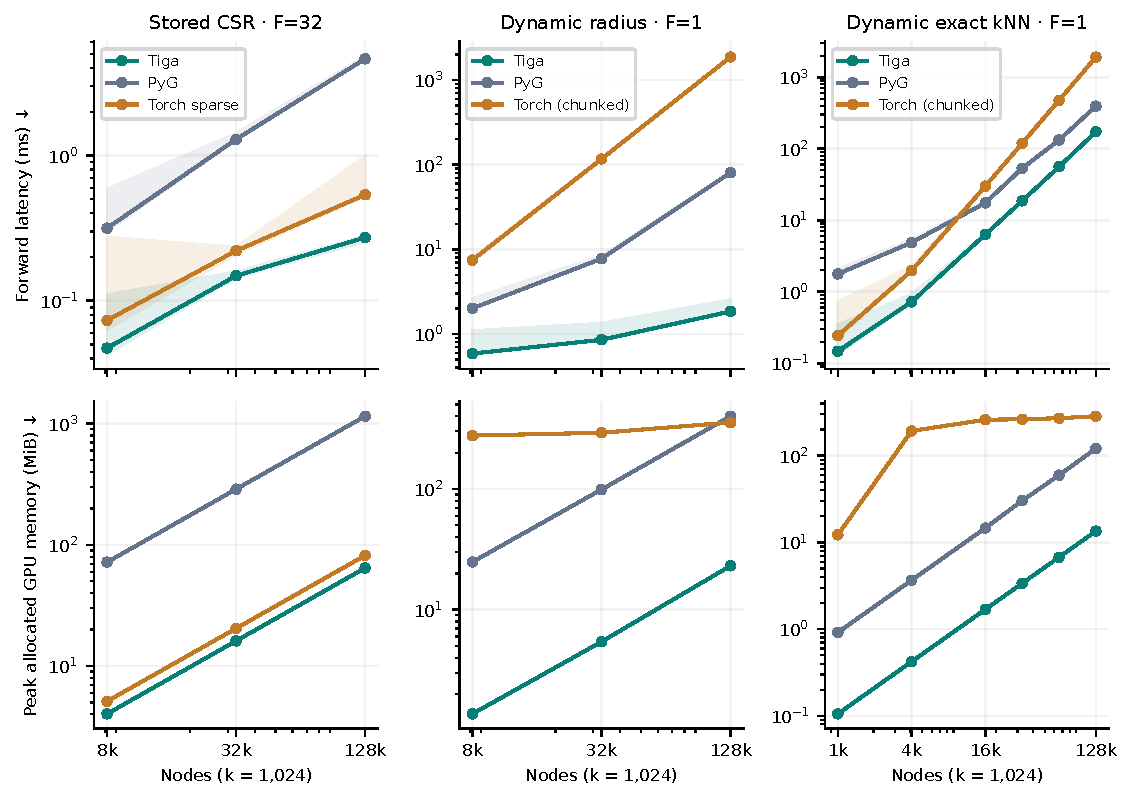
\includegraphics[width=\linewidth]{figures/q1-performance-memory.pdf}
\caption{Matched forward latency and measured allocated GPU memory.
Columns are different workloads; feature widths and sizes are not pooled.
Both rows use logarithmic axes and lower is better. Dynamic calls rebuild and
consume changed coordinates. Torch (chunked) means a pure Torch graph builder
and Torch aggregation, not a Tiga-built graph. kNN extends through 128K points;
the selected graph at that size has approximately 2.10M directed edges.}
\label{fig:q1}
\end{figure}

Stored CSR takes approximately 0.047--0.272 ms, giving 1.49--1.97$\times$
speedup over Torch sparse on the three measured sizes. Allocation is about
1.27$\times$ lower than the sparse peer, rather than the much larger reduction
against materialized COO messages. The largest dynamic radius case takes
1.84 ms versus PyG's 80.24 ms and pure Torch's 1,870.09 ms;
allocation peaks are 23.14, 400.22 and 355.01 MiB respectively.
These are workload-specific outcomes, not a framework ranking.

Exact kNN uses semantic executable rebinding and the exact tile-selection
pruning described in the compiler section. At 1,024 points Tiga takes 0.147 ms
versus 0.244 ms for pure Torch and 1.775 ms for PyG. At 16,384 points the
times are 6.32, 29.92 and 17.50 ms, respectively. At 131,072 points they are
172.37, 1,908.43 and 393.21 ms: Tiga is 2.28$\times$ faster than the PyG peer
with 13.50 versus 121.13 MiB allocated (pure Torch: 285.00 MiB).
Across the six measured sizes the PyG-relative speedup is 2.28--12.06$\times$.
All paths rebuild relations from changed coordinates; executable reuse does
not reuse selected neighbors. Candidate-distance work remains quadratic, so
these results do not establish subquadratic search or a universal advantage
over spatial-index kNN implementations.
\FloatBarrier

\subsection{Billion-edge execution on a single GPU}
\label{sec:billion}
The capacity workload is an explicit periodic directed CSR graph with 16
neighbors per destination and 32 FP32 features. Every edge is persisted and
traversed; the periodic closed-form oracle is used only for validation.
The sweep stops at 10M, 100M and 1B edges by design, not at a demonstrated
maximum supported size. Three fresh processes per size are retained from the
fully checked capacity run. Bounded ingest is untimed; forward includes
page loading, host staging, JIT as encountered, computation and output assembly,
but excludes full-output checking.

Pages contain 65,536 destination rows, prefetch is disabled, and the native
device budget is 12 GiB. This is a serialized capacity baseline, not a
measurement of overlapped IO or compiler-scheduled prefetch. The runtime's
optional read-ahead covers topology loading and contiguous field hints;
source gathering and GPU staging remain on the consuming thread. Enabling
that option alone does not create a disk--host--device double-buffered pipeline.
The final output remains resident. At 1B edges,
62.5M nodes require 8.5 GB of indices, 8 GB of source features and 8 GB of output.
The full-residency lower bound is 22.82 GiB with int64 CSR, or 18.86 GiB with
int32 CSR, both beyond 16 GiB. These are arithmetic infeasibility bounds, not
measured OOM attempts or Torch/PyG runs at this size. A hand-chunked peer could
also exchange storage traffic for capacity; paging is not claimed to be unique.

\begin{figure}[htbp]
\centering
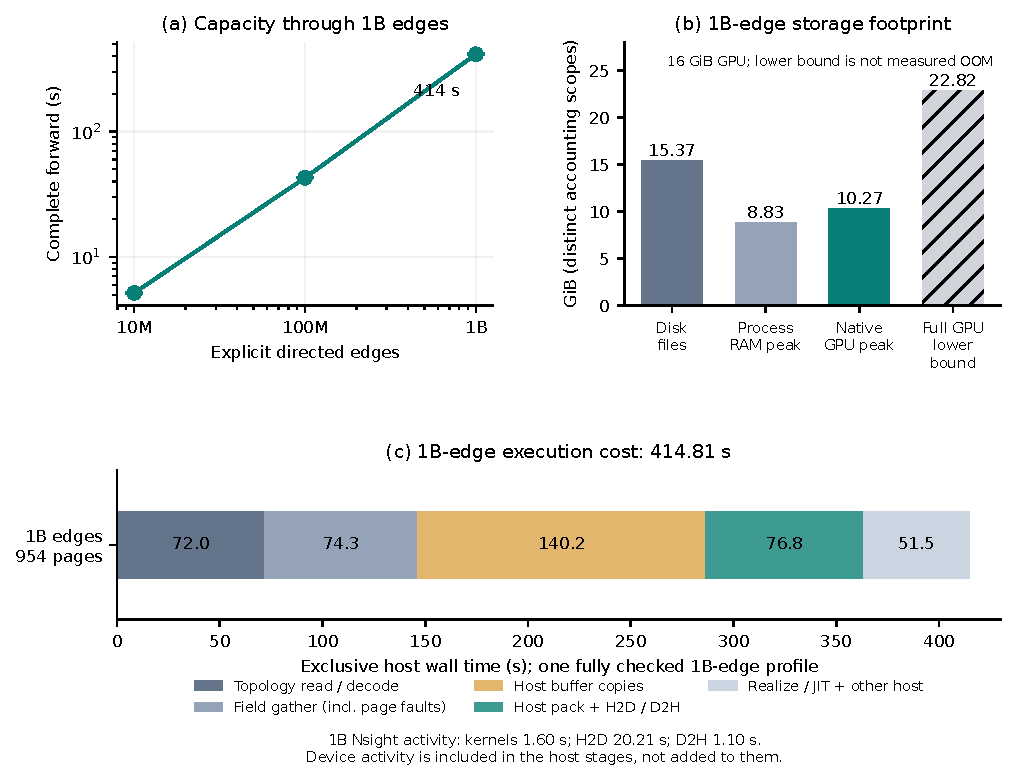
\includegraphics[width=\linewidth]{figures/q2-capacity-cost.pdf}
\caption{Single-GPU capacity and execution cost. (a) Median/range of three complete calls per size.
(b) Disk footprint, process RAM peak, native GPU peak and calculated full-residency
requirement at 1B, with distinct accounting scopes. (c) Exclusive host stages in
one fully checked, instrumented 1B-edge forward call. Nsight
CUDA activity is already contained in the host intervals, not an extra stage.}
\label{fig:q2}
\end{figure}

The 1B median is 414.25 seconds (411.36--415.61), with maximum native GPU peak
10.27 GiB and forward process RSS 8.83 GiB. All two billion output scalars are
checked exactly. Topology and source occupy 15.37 GiB on disk. Device-wide
sampled usage, including services and allocation pools, reaches 13.25 GiB;
the native counter alone is not total physical usage. The output occupies
7.45 GiB, so capacity still depends on node count and feature width.

A separate instrumented 1B-edge call records exclusive nested host intervals
and an Nsight CUDA capture restricted to forward. All two billion output
scalars are checked exactly afterward. The profiled window takes 414.81 seconds;
the outer call takes 417.05 seconds including profiler start/stop overhead.
It is not pooled into the original three-trial latency sweep.
Topology read/decode takes 71.98 seconds, field gathering 74.27 seconds,
host-buffer copying 140.22 seconds, packing and host/device transfer stages
76.79 seconds, and realization/setup/assembly 51.55 seconds.
These exclusive host intervals sum to the profiled window. Nsight separately
records 1.60 seconds of CUDA kernels, 20.21 seconds H2D and 1.10 seconds D2H;
these device activities are already contained in the host stages.

Host staging, rather than kernel arithmetic, dominates. Source staging expands
feature rows at edges: an 8 GB stored source field generates 128 GB of gathered
values. Total H2D traffic is 144.50 GB; D2H is 8 GB. Eviction hints on only the
three fixture files yield 16.50 GB of process physical reads, including any
runtime/compiler file reads. mmap gathering includes page-fault IO, not an
isolated disk-service timer. The graph fits host RAM; this is not evidence for
a graph beyond RAM capacity. CUDA paged backward, 1B recurrence and output
offload remain outside the demonstrated result.
\FloatBarrier

\subsection{Distributed execution and communication overhead}
\label{sec:two-host}
The 5070 Ti and 4070 Ti SUPER each own half the destination rows of one graph,
exchanging remote source features through halo maps. This is two-rank graph
partitioning, not feature-axis tensor parallelism or independent data-parallel
graphs. Ownership is fixed for each run.

The workload is a nonperiodic structured three-dimensional hexahedral mesh.
Nodes sharing an element are connected in both directions, excluding self
entries: an interior node has 26 neighbors, and exterior nodes have fewer.
This matches the connectivity of a trilinear hexahedral FEM discretization; the measured
operation is 16-feature neighbor summation, not stiffness assembly or a complete
FEM solve. Cubes have side lengths 32, 64 and 96, giving 32,768, 262,144 and
884,736 nodes and 797,816, 6,596,856 and 22,508,920 directed edges.

Lexicographic x-major numbering makes the equal-row partition a spatial plane.
Each rank owns half the volume and exchanges one interface layer rather than
a volume-sized ghost set. For a cube of side length L,
$$
N=L^3,\qquad N_{\mathrm{halo,rank}}=L^2,\qquad
f_{\mathrm{boundary}}=\frac{2}{L}.
$$
The boundary
fractions decrease from 6.25\% to 3.125\% and 2.083\%; total traffic across both
ranks is 0.125, 0.500 and 1.125 MiB per call. Thus the experiment measures the
small surface-to-volume regime relevant to spatial graphs.

Each GPU also executes the complete graph alone. The \emph{communication then
compute} schedule completes halo exchange before computing local outputs.
Two warmups precede five changed-input, fully checked calls. Per-sample distributed latency
is the maximum of paired rank durations, followed by a median, not the mean of
rank medians. Topology setup, input allocation, the control barrier and checking
are excluded. Setup topology is replicated and partition maps cached: this is
strong scaling, not distributed topology-capacity evidence beyond one GPU.

Both hosts use matching Tiga sources and compiler executables.
Single-card and two-card modes share the native-input timing boundary; their
times are not directly comparable with the different ordinary-Torch workloads
in Section~\ref{sec:performance}.
Modes run in fixed order; small sample counts and shared services limit
cross-run generalization.

\begin{figure}[htbp]
\centering
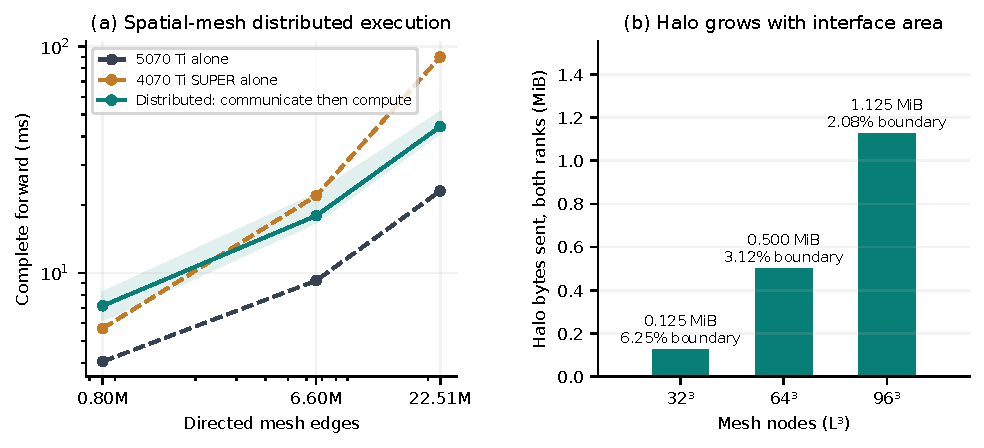
\includegraphics[width=\linewidth]{figures/q3-distributed.pdf}
\caption{Distributed NCCL execution of spatial mesh graphs on two hosts.
(a) Full-graph single-GPU baselines and paired two-rank latency.
(b) Halo traffic grows with the interface area while the boundary fraction
shrinks with mesh size. Latency covers the complete forward call: halo exchange,
runtime scheduling, computation and synchronization. Each rank owns half the destination nodes.}
\label{fig:q3}
\end{figure}
At 22.51M directed edges, the 5070 Ti and 4070 Ti SUPER single-GPU medians are 23.00 and 89.75 ms. The communication-then-compute schedule takes 44.22 ms on the paired-rank critical path, 1.92 times the faster single-GPU latency. Only 2.08\% of each rank's destination rows touch the interface, and total halo traffic is 1.125 MiB. This fixed partition assigns half the destination rows to each GPU. Compute-aware partitioning is a potential optimization for the measured heterogeneous pair.

\FloatBarrier

\subsection{Reproduction and scope}
\path{data/comparison-v3/} stores the 36 comparison records, source snapshot
and allocation audits. \path{data/billion/} contains the nine capacity trials;
\path{data/paging-1b/} contains the instrumented billion-edge run and Nsight capture.
\path{data/distributed-spatial/} contains both rank records, commands, source
and interface-size checks for the spatial-mesh experiment.
\path{tools/build_three_questions.py} validates the archived configurations and
numerical checks before plotting. Rerunning hardware measurements uses the commands
and environments provided with each dataset.

The results establish path-specific speed/memory improvements, 1B single-GPU
capacity and measured two-host overhead. They do not establish universal PyG
superiority, an absolute maximum edge count, distributed speedup, full-training
throughput or isolated NVMe service time.
